\documentclass[a4paper]{article}
\usepackage{graphicx} % Required for inserting images
\usepackage[margin = 2.8cm]{geometry} 
\usepackage{palatino}
\usepackage{listings}
\usepackage{xcolor}
\usepackage{hyperref}

\lstdefinestyle{mypython}{
  language=Python,
  basicstyle=\ttfamily\footnotesize,
  keywordstyle=\color{green}\bfseries,
  stringstyle=\color{blue},
  commentstyle=\color{gray}\ttfamily\itshape,
  showstringspaces=false,
  breaklines=true
}

\lstset{style=mypython}

\title{ELEC0447 -- Project 1 \\ Low voltage distribution feeder modeling and analysis}
\author{Bertrand Corn\'elusse}
\date{October 2, 2026, version 1.0}

\begin{document}

\maketitle

\begin{center}
    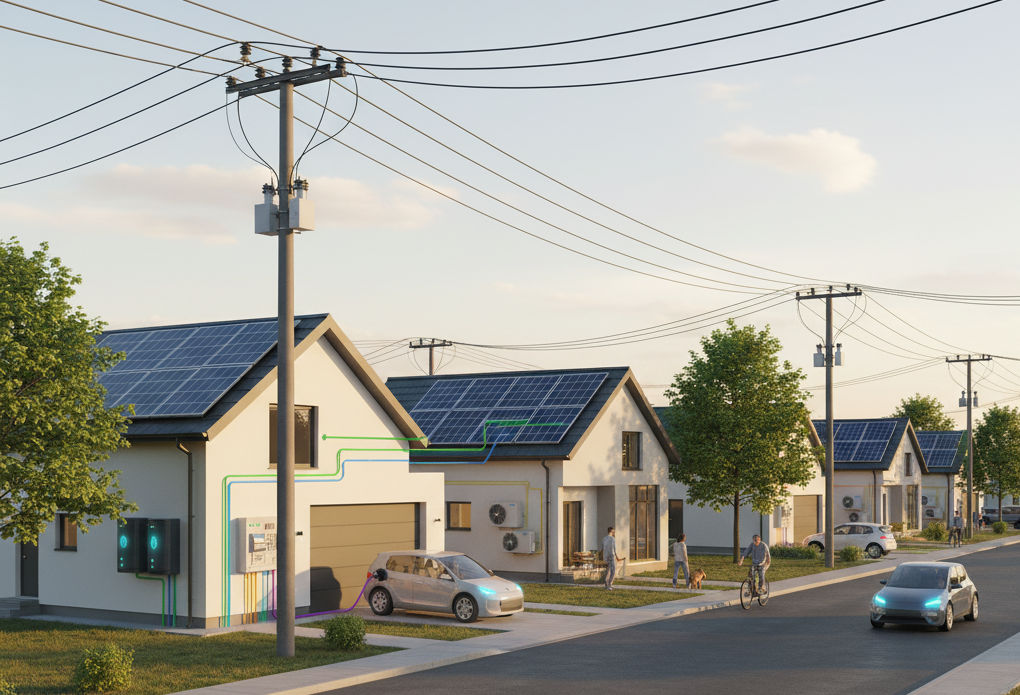
\includegraphics[width=0.99\linewidth]{Gemini_Generated_Image_djxmz2djxmz2djxm.png}
    Image generated by Google Gemini (what's wrong with this picture?) 
\end{center}

\section{Introduction}
The goals of this assignment are to
\begin{enumerate}
    \item get familiar with Python and PandaPower, a power system modeling tool
    \item learn to run some first power-flow analyses on a simple network
    \item gain some intuition on the impact of high loads and renewable distributed generation
    \item compare three-phase balanced and unbalanced operating conditions.
\end{enumerate}

Let's consider a street where two distribution network feeders connect ten houses. A \textit{feeder} is a power line that carries electricity from a substation or distribution transformer, which we will model as our slack bus, to the end-users. 
The network data is provided as an Excel file with separate sheets that describe the buses, lines, and loads.

\begin{center}
\textit{Remark: we used PandaPower version 3.1.2 to carry out all the experiments below.}   
\end{center}

\newpage

\section{Your tasks}
\begin{enumerate}
\item \textbf{(Base case)} Write a Python code to model a \textbf{single-phase equivalent }of the network and run a first power flow analysis\footnote{An example code for a 3-bus network is available as a link in the slides on the power flow analysis. You can use it as a starting point. You should also consult PandaPower's documentation.}.
\item Explore the results of the base case. Plot the network schematic and the voltage magnitude and angle evolution along the feeders. Display the line loading coefficients. Briefly discuss the results.
\item Starting from the base case, progressively increase the load (keep the same power factor) at the buses near the end of the feeder (this simulates the addition of electric vehicles or heat pumps). What do you observe? Is there a loading condition such that the power flow does not converge? Explain.
\item Starting from the base case, add photovoltaic plants at the buses near the end of the feeders and progressively increase their production (from 1 to 10kW). What do you observe? 
\item \textbf{(3-phase base case)} Now, you will model the network more accurately using a model of the three phases. Update the model to run a three-phase power flow. 
\begin{enumerate}
\item First, update the cable type to encode the \textit{zero-sequence parameters}\footnote{This is to model the coupling between the phases. You must not fully understand what is done here, browse the internet if you want to know more.} of the line
\begin{lstlisting}[language=Python, caption=Updating the cable type.]
import pandapower as pp
pp.create_std_type(net, {"r_ohm_per_km": 0.642, "x_ohm_per_km": 0.083,
                "c_nf_per_km": 210., "max_i_ka": 0.142,
                "endtemp_degree": 70.0, "r0_ohm_per_km": 1.923,
                "x0_ohm_per_km": 0.249,
                "c0_nf_per_km":  70}, name="unsymmetric_NAYY 4x50 SE",element = "line")
line_type = "unsymmetric_NAYY 4x50 SE" # To be used when creating the lines.
\end{lstlisting}
and then use this line type to create the lines.
\item Using the function \lstinline{pp.create_asymmetric_load}, load the system so that you are \textbf{in the same conditions than in the base case }(with the \textbf{single-phase equivalent }). Use star (or wye) connected loads.
\item Add the following commands to run the power flow\footnote{Again, no need to understand everything, it is required to make it work.}:
\begin{lstlisting}[language=Python, caption=Running a three-phase power flow analysis.]
net.ext_grid['s_sc_max_mva'] = 1000
net.ext_grid['rx_max'] = 0.1
pp.add_zero_impedance_parameters(net)
pp.pf.runpp_3ph.runpp_3ph(net, algorithm='nr', calculate_voltage_angles=True)
\end{lstlisting}
\item If it succeeds, you can now access the results in the \lstinline|net| object (e.g. \lstinline{net.res_bus_3ph.vm_a_pu}).
\end{enumerate}
\item Explore the results of the 3-phase base case. Plot the evolution of the magnitudes and angles of the voltage along the feeder (from bus 0 to bus 10). Display the currents in the phases and the neutral along the feeder. Briefly discuss the results.
\item Starting from the 3-phase base case, load the network so that the total load at each bus is equally shared between phase a and phase b. What can you observe?
\item Start from the 3-phase base case. By chance, all homeowners connected a 2 kVA photovoltaic inverter on phase a. Model this situation when the inverters all produce the maximum active power. What do you observe? What could you do to improve the situation? Note: a photovoltaic inverter is indivisible.
\item Simulate the situation where 
\begin{enumerate}
    \item a 3-phase fault cuts the line between the transformer and the first bus of the first feeder; 
    \item The line connecting the ends of the two feeders is activated.
\end{enumerate}
Repeat the last analysis with the inverters on phase a.
\end{enumerate}

\section{Organization and Evaluation} 
\begin{enumerate}
    \item \textbf{Project preparation:} You are encouraged to prepare the project in \textbf{groups of 2} (working individually is also permitted as a choice). However, \textbf{the evaluation itself will be strictly individual}.
    
    \item \textbf{No written report:} There is \textbf{no written report} to submit for this project.
    
    \item \textbf{Code submission:} You must submit your working Python notebook or scripts (as a \texttt{.zip} archive if multiple files) on \textbf{eCampus} by \textbf{November 4, 2026, at 23:59}.
    
    \item \textbf{Live evaluation session:} 
    \begin{itemize}
        \item The project evaluation will take place in person on \textbf{November 5, 2026} (during the scheduled course session; presence is mandatory).
        \item The evaluation is \textbf{individual}: each student will be interviewed and assessed separately.
        \item Each student must bring a laptop with a fully working, ready-to-run implementation of all 9 tasks, and an environment properly configured (Python, PandaPower, matplotlib, etc.) without relying on an internet connection or facing installation delays.
    \end{itemize}
    
    \item \textbf{Evaluation format and requirements:} During the individual defense, the evaluation team will interact with you based on your live code:
    \begin{itemize}
        \item \textbf{Live figure and analysis regeneration:} You will be asked to rerun parts of your code and regenerate specific figures, curves, or analyses on the fly, and physically interpret the results.
        \item \textbf{High-quality visualization:} Your plots must be clear, readable, and properly formatted (labeled axes, physical units, legends) $\rightarrow$ see the \href{https://www.youtube.com/watch?v=rUV8VFbUi_U}{tutorial video on plotting in Python}.
        \item \textbf{Live on-the-spot code modifications:} To test your understanding and code mastery, the evaluation team will ask you to make small live modifications. These changes will require at most \textbf{2 to 3 lines of code} in a clean implementation. For instance, you might be asked to:
        \begin{itemize}
            \item add a bus and a line chunk to connect it to an existing feeder;
            \item modify loading conditions (e.g., scale load values, alter power factors, or change phase allocations);
            \item adjust photovoltaic production levels or redistribute inverters;
            \item simulate a line disconnection or an alternative feeder interconnection.
        \end{itemize}
    \end{itemize}
    
    \item \textbf{Practical advice for success:}
    \begin{itemize}
        \item Structure your code modularly using functions or parameterized blocks rather than long monolithic scripts, so that network elements, loads, and generation can be updated in 2--3 lines without rewriting your scripts.
        \item Make sure you personally understand and can explain every part of the implementation, even if you divided the preparation work with your partner.
        \item Verify beforehand that your entire notebook or script can be executed sequentially from scratch without errors or long recalculation times.
    \end{itemize}
\end{enumerate}

\end{document}
